% Define document class
\documentclass[twocolumn]{aastex631}

% Filler text
\usepackage{blindtext}

\newcommand{\tess}{\textit{TESS}}
\newcommand{\sname}{V1298~Tau}
\newcommand{\allplanets}{V1298~Tau~bcd}
\newcommand{\planetb}{V1298~Tau~b}
\newcommand{\planetc}{V1298~Tau~c}
\newcommand{\planetd}{V1298~Tau~d}
\newcommand{\planete}{V1298~Tau~e}
\newcommand{\rearth}{$R_\oplus$}
\newcommand{\exoplanet}{\texttt{exoplanet}}




% Begin!
\begin{document}

% Title
\title{Updated Ephemerides of the young multi-planet system V1298 Tau from TESS}

% Author list
\author[0000-0002-9464-8101]{Adina~D.~Feinstein}
\altaffiliation{NSF Graduate Research Fellow}
\affiliation{Department of Astronomy and Astrophysics, University of Chicago, Chicago, IL 60637, USA}

\author[0000-0001-6534-6246]{Trevor J.\ David}
\affiliation{Center for Computational Astrophysics, Flatiron Institute, New York, NY 10010, USA}
\affiliation{Department of Astrophysics, American Museum of Natural History, New York, NY 10024, USA}

\author[0000-0001-7516-8308]{Benjamin~T.~Montet}
\affiliation{School of Physics, University of New South Wales, Sydney, NSW 2052, Australia}
\affiliation{UNSW Data Science Hub, University of New South Wales, Sydney, NSW 2052, Australia}

\author[0000-0002-4881-3620]{John~H.~Livingston}
\affiliation{Department of Astronomy, University of Tokyo, 7-3-1 Hongo, Bunkyo-ku, Tokyo 113-0033, Japan}

\author{Charles Beichman}
\affiliation{Caltech/IPAC, 1200 E. California Blvd. Pasadena, CA 91125, USA}


\author[0000-0002-3199-2888]{Sarah Blunt}
\altaffiliation{NSF Graduate Research Fellow}
\affiliation{Department of Astronomy, California Institute of Technology, Pasadena, CA, USA}


\author{DFM?}

\correspondingauthor{Adina~D.~Feinstein;\\ \twitter{afeinstein20}; \github{afeinstein20};} \email{afeinstein@uchicago.edu} 

% Abstract with filler text
\begin{abstract}
  \sname is a young ($\sim$23~Myr) solar analogue hosting four transiting exoplanets. 
  Given its planets range between 0.5 - 0.9 $R_J$, this system provides a unique opportunity to 
  understand the evolution of planetary radii in the same stellar environment. \sname was originally 
  observed 6 years ago during K2 Campaign 4. The extended mission of NASA's Transiting Exoplanet Survey 
  Satellite (\tess) includes observing the ecliptic plane. Here, we present new photometric observations 
  of \sname from the 10-minute TESS Full-Frame Images. We use the TESS data to update the transit-timing 
  for \allplanets as well as compare newly observed radii to that derived from the K2 light curve. We 
  additionally catch a transit of \planete, which was a single-transit event in the previous data, allowing 
  us to further constrain the period of this farthest known planet. \sname is the target of several ongoing 
  and future observations, including with the James Webb Space Telescope. These updated ephemerides will be 
  crucial for accurately recovering transit events and understanding any future doppler tomographic or 
  transmission spectroscopy signals.

\end{abstract}

% Main body with filler text
\section{Introduction}


%%%%%%%%%%%%%%%%%%%%%%%%%%%%%%%%%%%%%%%%%%%%%%%%%%%
\begin{figure*}[!ht]
\begin{center}
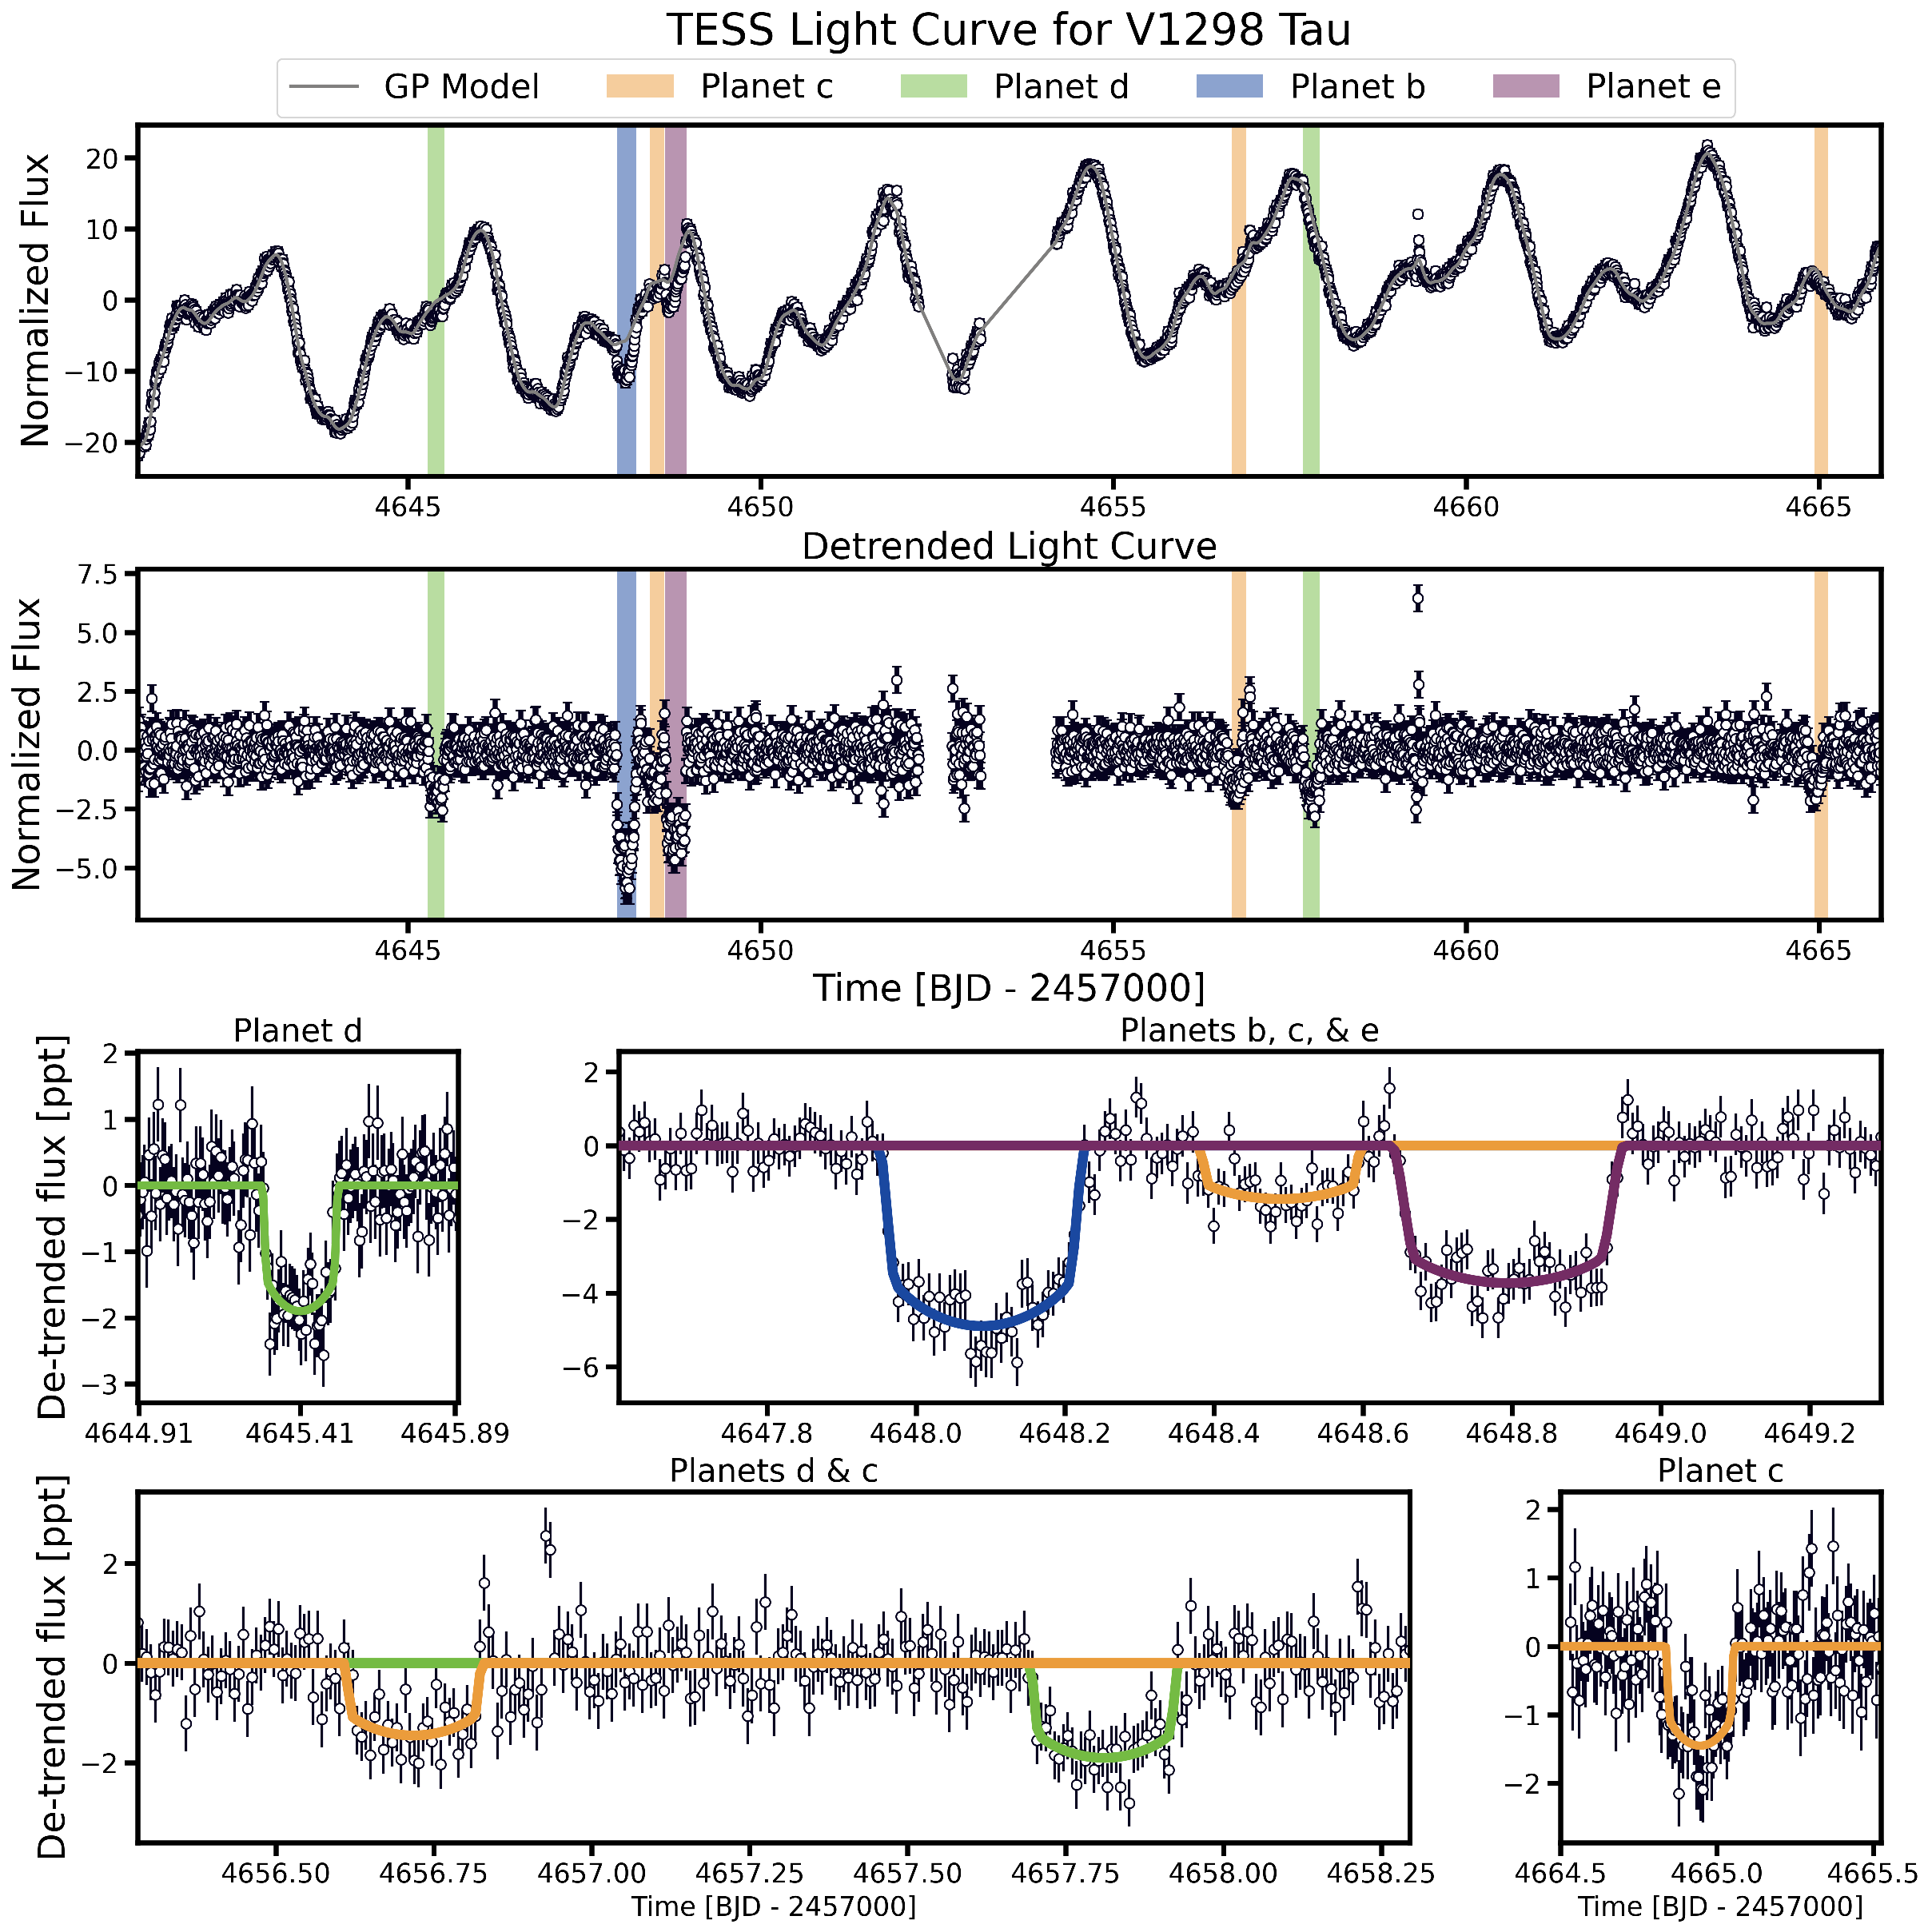
\includegraphics[width=\textwidth,trim={0.25cm 0 0 0}]{static/lightcurve.pdf}
\caption{\sname extracted light curve from the \texttt{tica}-processed full-frame images, with transits of \allplanets highlighted by color. Top row: extracted light curve with over plotted with our best-fit GP model for stellar variability (black). Middle row: the \tess\ light curve with the stellar variability removed by our model. Bottom rows: zoomed-in regions around the visible transits during the first orbit (third row) and second orbit (last row) from \tess\ Sector 43. \label{fig:transits}}
\end{center}
\end{figure*}
%%%%%%%%%%%%%%%%%%%%%%%%%%%%%%%%%%%%%%%%%%%%%%%%%%%

\end{document}
